\documentclass{beamer}
\usepackage{multicol}
\usepackage{xy}
\everymath{\displaystyle}
\mode<presentation>
{\usetheme{Warsaw}\setbeamercovered{dynamic}}
\usecolortheme{crane}
\usepackage{beamerfoils}
\pgfdeclareimage[height=1in]{university-logo}{ISULogo}
\logo{\pgfuseimage{university-logo}}
\setbeamertemplate{navigation symbols}{}
\title[\S10]{Section 10\\Combinatorics applications}
\author{Dr Marcus Bishop}
\subject{Math 104}
\beamerdefaultoverlayspecification{<+->}
\theoremstyle{definition}
\newtheorem{remark}{Remark}
\newtheorem{impact}{Impact}
\newtheorem{situation}{Situation}
\newtheorem{question}{Question}
\usepackage{arev}
\usepackage{tensor}
\newcommand\npr[2]{\tensor[_{#1}]P{_{#2}}}
\newcommand\ncr[2]{\tensor[_{#1}]C{_{#2}}}
\usepackage{cancel}
\newcommand{\hs}{\alert{\varheart}}
\newcommand{\ds}{\alert{\vardiamond}}
\newcommand{\s}{\spadesuit}
\newcommand{\cs}{\clubsuit}
\begin{document}
\begin{frame}\titlepage\end{frame}
\LogoOff

\begin{frame}{Poker outline}
\begin{itemize}
\item Dealer deals five cards from standard deck
to each player
\item Selection of five cards called a \alert{hand}
\item For simplicity, we imagine all five cards in player's hand
\item In reality, some cards lying face up on table
\item Players make bets and/or replace cards
\item Finally, player with \alert{best hand} wins
\item Nine categories of poker hands:
\begin{tabular}{lll}
Straight flush&Four-of-a-kind&Full house\\
Flush&Straight&Three-of-a-kind\\
Two pairs&One pair&High card
\end{tabular}
\item Strength of hand determined by its probability
%(although listed from best to worst above)
\item The smaller the probability, the stronger the hand
\item If two players have same type of hand, tie
broken in manner depending on type of hand
\end{itemize}
\end{frame}

\begin{frame}{Playing cards}
\begin{itemize}
\item Recall that deck has cards of thirteen \alert{ranks},
$A,K,Q,J,10,9,8,7,6,5,4,3,2$
listed from highest to lowest
\item Each rank has four cards, one of each \alert{suit} $\hs,\ds,\cs,\s$
\item Thus deck has $13\cdot 4=52$ cards
\end{itemize}
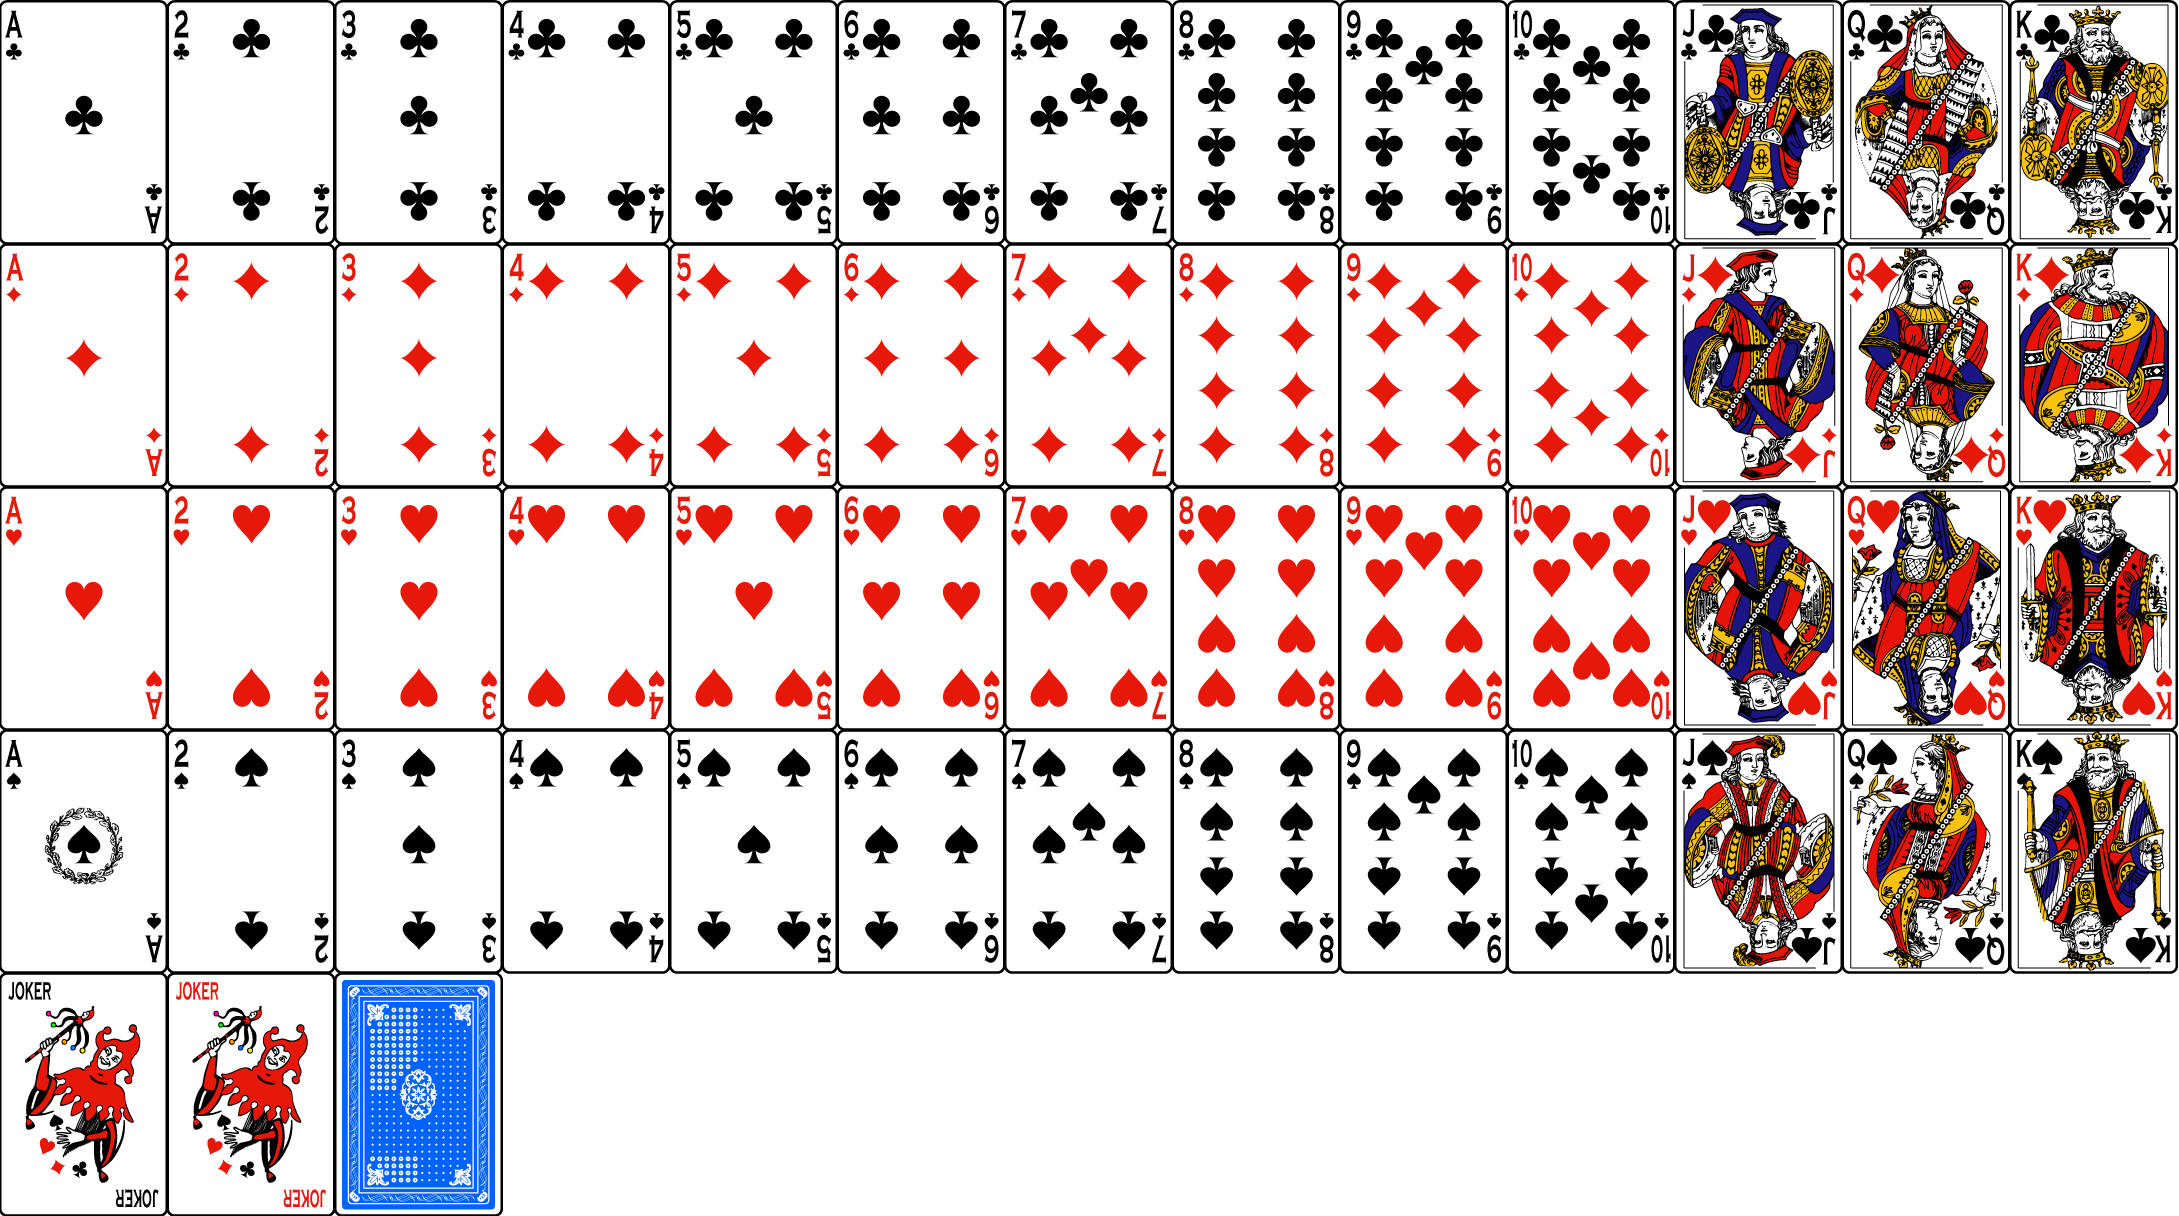
\includegraphics[scale=.3]{cards}
\end{frame}

\begin{frame}{Poker basics}
\begin{itemize}
\item So $\ncr{52}{5}=2,598,960$ the number of possible hands
\item Will first calculate probability that player dealt
hand of particular type
\item This probability not altered by fact that other cards
might have already been dealt to other players
\item \dots provided that those cards \alert{not exposed to player}
\item However, some variants of poker involve exposing cards
\end{itemize}
\begin{example}
If card of suit $\hs$ lying face up on table, affects probability
that next card drawn will have suit $\hs$
\end{example}
\end{frame}

\begin{frame}{Four of a kind}
\begin{itemize}
\item Hand called \alert{four-of-a-kind} if four cards have
same rank
\item Fifth card and common rank of first four cards unimportant
\item However, if another player also has four-of-a-kind,
then player with four cards of highest rank wins
\begin{example} $8\hs,8\ds,8\cs,8\s,10\cs$ a four-of-a-kind\end{example}
\begin{example} $9\hs,9\ds,9\cs,9\s,3\hs$ a four-of-a-kind,
beats hand above\end{example}
\end{itemize}
\end{frame}

\begin{frame}{Counting four-of-a-kinds }
\begin{itemize}
\item How many ways to form four-of-a-kind?
\item Thirteen ways to choose common rank of four cards
\item $52-4=48$ cards remain
\item So $48$ ways to choose fifth card
\item Thus $13\cdot 48=624$ possible four-of-a-kinds
\item So $\frac{624}{2598960}=\frac{1}{4165}\approx 0.00024$
the probability of being dealt four-of-a-kind
\end{itemize}
\end{frame}

\begin{frame}{Full house}
\begin{itemize}
\item Hand called a \alert{full house} if three
cards have same rank and remaining two have same rank
\begin{example} $8\hs,8\ds,8\cs,10\s,10\ds$ a full house,
an \alert{eights-over-tens full house}\end{example}
\item If another player has full house, then player with
three cards of highest rank wins
\begin{example} $9\hs,9\ds,9\cs,7\hs,7\s$ a full house,
a \alert{nines-over-sevens full house},
beats hand above\end{example}
\end{itemize}
\end{frame}

\begin{frame}{Counting full houses}
\begin{itemize}
\item First choose two common ranks
\item $13$~ways to choose first rank
\item $12$~ways to choose second rank
\item Next, choose three cards of first rank
\item $\ncr{4}{3}=4$ ways
\item Finally, choose two cards of second rank
\item $\ncr{4}{2}=6$ ways
\item So $13\cdot 12\cdot 4\cdot 6=3744$ possible full houses
\item So $\frac{3744}{2598960}=\frac{6}{4165}\approx 0.00144$
the probability of begin dealt full house
\item Note that $\frac{6}{4165}>\frac{1}{4165}$,
so four-of-a-kind beats full house
\end{itemize}
\end{frame}

\begin{frame}
\newcommand{\bl}{\underline{\hspace{3mm}}}
\begin{example} $8\hs,8\ds,8\cs,10\s,10\ds$ a full house\end{example}
\begin{itemize}
\item $13\cdot 12\cdot\ncr{4}{3}\cdot\ncr{4}{2}$ possible full houses
(see previous slide)
\item $13$ choices for first rank, $8$ in example above
\item At this stage, have chosen
$8\bl,8\bl,8\bl,\bl\;\bl,\bl\;\bl$
\item $12$ choices for second rank, $10$ in example
\item At this stage, have chosen
$8\bl,8\bl,8\bl,10\bl,10\bl$
\item $\ncr{4}{3}$ choices of suits of cards of first
rank, $\hs,\ds,\cs$ in example
\item At this stage, have chosen
$8\hs,8\ds,8\cs,10\bl,10\bl$
\item $\ncr{4}{2}$ choices of suits of cards of second
rank, $\s,\ds$ in example
\item At this stage, have chosen
$8\hs,8\ds,8\cs,10\s,10\ds$
\end{itemize}
\end{frame}

\begin{frame}{Two-pair}
\begin{itemize}
\item Hand called \alert{two-pair} if two
cards have same rank and another two have same rank
\item Rank of second pair should be different than rank of first,
else hand a four-of-a-kind
\item Fifth card should have rank different than ranks
of remaining cards, else hand a full house
\end{itemize}
\end{frame}

\begin{frame}
\begin{itemize}
\begin{example} $2\hs,2\ds,Q\cs,Q\s,10\ds$ a two-pair\end{example}
\item If another player has two-pairs, tie broken
by comparing highest ranking pairs
\begin{example} $K\s,K\hs,7\ds,7\s,A\s$ a two-pair,
beats hand above, since $K$ higher than $Q$\end{example}
\item If two players have
highest ranking pair of same rank, then tie broken
by comparing lowest ranking pairs
\begin{example} $K\cs,K\ds,J\hs,J\cs,3\hs$ a two-pair,
beats both hands above\end{example}
\end{itemize}
\end{frame}

\begin{frame}{Counting two-pairs}
\begin{itemize}
\item First choose two common ranks
\item $\ncr{13}{2}=78$~ways to choose ranks
\item Next, choose two cards of first rank
\item $\ncr{4}{2}=6$ ways
\item Next, choose two cards of second rank
\item $\ncr{4}{2}=6$ ways
\item Finally, choose fifth card
\item $52-8=44$ remaining cards have ranks different
than ranks chosen above
\item So $78\cdot 6\cdot 6\cdot 44=123,552$ possible two-pairs
\item So $\frac{123552}{2598960}=\frac{198}{4165}\approx 0.04754$
the probability of begin dealt two-pair
\end{itemize}
\end{frame}

\begin{frame}
\begin{itemize}
\item But why were common ranks chosen with $\ncr{13}{2}$
but with $13\cdot 12$ in full house calculation?
\item Because in full house, one common rank has \alert{three}
cards, while other common rank has \alert{two}
\item In two-pair, $13\cdot 12$ would have counted
each hand \alert{twice}
\item So we instead used
$\ncr{13}{2}=\frac{13\cdot 12}{2!}$
\item $2!$ in denominator accounts for duplication
\item Analogous to factorials in denominator of
anagram calculation
\begin{example}
\begin{itemize}
\item Word \alert{book} has
$\frac{4!}{2!}=12$ anagrams
\item Role of $2!$ to eliminate duplicate anagrams
resulting from swapping o's
\end{itemize}
\end{example}
\end{itemize}
\end{frame}

\begin{frame}{Three-of-a-kind}
\begin{itemize}
\item Hand called \alert{three-of-a-kind} if
three cards have same rank
\item Remaining two cards should have rank different
than first three (else hand is four-of-a-kind)
\item Also, remaining cards should have rank
different than one another (else hand is full house)
\begin{example} $8\hs,8\ds,8\cs,Q\hs,10\cs$ a three-of-a-kind\end{example}
\end{itemize}
\end{frame}

\begin{frame}{Counting three-of-a-kinds}
\begin{itemize}
\item $13$ choices for common rank of three cards
\item $\ncr{4}{3}=4$ choices for three cards of rank chosen above
\item $52-4=48$ cards have rank different than rank chosen above
\item So $48$~choices for fourth card
\item $48-4=44$~cards have rank different than two ranks chosen above
\item So $44$~choices for fifth card
\item However, order in which fourth and fifth cards selected unimportant
\item $48\cdot 44$ counts each choice \alert{twice}
\item Hence divide final answer by $2$
\item So $\frac{13\cdot 4\cdot 48\cdot 44}{2}=54,912$ three-of-a-kinds
\end{itemize}
\end{frame}

\begin{frame}{Another way to count three-of-a-kinds}
\begin{itemize}
\item $13$ choices for common rank of three cards
\item $\ncr{4}{3}=4$ choices for three cards of rank chosen above
\item $\ncr{12}{2}=66$ choices for ranks of two remaining cards
\item $4$~choices for suit of fourth card 
\item $4$~choices for suit of fifth card 
\item So $13\cdot 4\cdot 66\cdot 4\cdot 4=54,912$ three-of-a-kinds
\item Agrees with previous calculation
\item So $\frac{54912}{2598960}=\frac{88}{4165}\approx 0.02113$ the probability
of being dealt four-of-a-kind
\end{itemize}
\end{frame}

\begin{frame}
\begin{situation}
\begin{itemize}
\item You have $3\hs,8\hs,J\hs,Q\hs,5\s$
\item Would like to replace $5\s$ with card of suit $\hs$ to complete flush
\item You know your opponent has two-pair (by telepathy or otherwise)
\item You surmise she would like to exchange fifth card to complete full house
\end{itemize}
\end{situation}
\begin{itemize}
\item $52-5=47$ cards remain unknown to you
\item You have four $\hs$'s so nine $\hs$'s remain
\item So you receive $\hs$ with probability $\frac{9}{47}$
\item But $\frac{9}{47}$ \alert{not} your probability of winning!
\item Opponent must also \alert{fail} to complete her full house,
since full house beats flush
\end{itemize}
\end{frame}

\begin{frame}
\begin{itemize}
\item Opponent has two pairs
\item For concreteness, suppose she has $4\s,4\cs,5\ds,5\s$
\item So she completes full house if she receives $4$ or $5$
\item So she \alert{fails} to complete full house
if rank of card dealt not $4$ \alert{and} not $5$
\item Since she has two $4$'s, two remain unknown to her
\item Since has two $5$'s, two remain unknown to her
\item So $47-2-2=43$ unknown cards are not $4$ and not $5$
\item Thus $\frac{43}{47}$ her probability of \alert{failing}
\item So $\frac{9}{47}\cdot\frac{43}{47}\approx 0.1752$
your probability of winning
\end{itemize}
\end{frame}

\begin{frame}
\begin{situation}
\begin{itemize}
\item You have $J\hs,J\cs,4\s,4\hs,Q\cs$
\item You could exchange $Q\cs$, hoping to complete full house
\item You could also exchange $4\s,4\hs,Q\cs$, hoping to build better hand
\end{itemize}
\end{situation}
\begin{itemize}
\item Suppose you exchange $Q\cs$
\item Two of $47$ cards unknown to you are jacks, two are $4$'s
\item Thus $\frac{4}{47}=\frac{1}{12}\approx 0.0851$ your probability
of completing full house
\end{itemize}
\end{frame}

\begin{frame}
\begin{itemize}
\item Suppose instead you exchange $4\s,4\hs,Q\cs$
\item First calculate probability that exactly one of new cards
a jack
\item Then you have three-of-a-kind
\item Additionally, if last two cards have same rank,
then you have full house, a \alert{jacks-over-something full house}
\item $47$ cards remain unknown to you, two of which jacks
\item So $45$ unknown cards have rank other than jack
\item Want to receive one jack and two non-jacks
\item Could happen in three ways, since jack could be
first, second, or third card
\item So $\frac{45}{47}\cdot\frac{44}{46}\cdot\frac{2}{45}
+\frac{45}{47}\cdot\frac{2}{46}\cdot\frac{44}{45}
+\frac{2}{47}\cdot\frac{45}{46}\cdot\frac{44}{45}\approx 0.1221$
the probability of jacks-over-something full house
\end{itemize}
\end{frame}

\begin{frame}
\begin{itemize}
\item Assuming you exchange $4\s,4\hs,Q\cs$
might instead receive \alert{two} jacks
\item Then you have four-of-a-kind
\item $47$ cards remain unknown to you, two of which jacks
\item So $45$ unknown cards have rank other than jack
\item Then \[\frac{45}{47}\cdot\frac{2}{46}\cdot\frac{1}{45}
+\frac{2}{47}\cdot\frac{45}{46}\cdot\frac{1}{45}
+\frac{2}{47}\cdot\frac{1}{46}\cdot\frac{45}{45}
=\frac{3}{1081}\approx 0.0028\]
your probability of four-of-a-kind
\end{itemize}
\end{frame}

\begin{frame}
An alternate four-of-a-kind calculation:
\begin{itemize}
\item You discard $4\s,4\hs,Q\cs$ and receive three new cards
\item $47$ cards remain unknown to you, two of which jacks
\item $\ncr{47}{3}=16,215$ ways to receive $3$ cards from remaining $47$
\item How many combinations have two jacks?
\item If two cards are jacks, then third card not a jack
\item $45$ non-jacks remain, so $45$ combinations
have two jacks
\item Thus $\frac{45}{16215}=\frac{3}{1081}\approx 0.0028$
the probability of four-of-a-kind
\end{itemize}
\end{frame}

\begin{frame}
\begin{itemize}
\item Assuming you exchange $4\s,4\hs,Q\cs$
might instead receive three cards of same rank
\item Then you have \alert{something-over-jacks full house}
\item First choose common rank of three cards
\item $10$ ways to choose rank other than $J,4,Q$
\item Then choose three cards of this rank
\item $\ncr{4}{3}=4$ ways to choose cards
\item So $10\cdot 40$ ways to choose three cards of
same rank other than $J,4,Q$
\item Also, three queens remain, so $41$ ways
to choose three cards of same rank
\item $\ncr{47}{3}=16,215$ possible ways to
choose three of remaining $47$ cards
\item Thus $\frac{41}{16215}\approx 0.0025$
your probability of something-over-jacks full house
\end{itemize}
\end{frame}

\begin{frame}
An alternate something-over-jacks calculation:
\begin{itemize}
\item $40$ of remaining $47$ cards of rank different than $J,4,Q$
\item So $\frac{40}{47}$ the probability of drawing
a card of rank different than $J,4,Q$
\item Afterwards three of remaining $46$ cards have same rank as first card
\item Afterwards two of remaining $45$ cards have same rank
as first two
\item So $\frac{40}{47}\cdot\frac{3}{46}\cdot\frac{2}{45}
=\frac{8}{3243}\approx 0.0025$ the probability
of drawing three cards of same rank
\item Note that calculation on previous slide includes
possibility of receiving $Q\hs,Q\ds,Q\s$, excluded from this calculation
\end{itemize}
\end{frame}

\begin{frame}{Summary}
\begin{itemize}
\item You have $J\hs,J\cs,4\s,4\hs,Q\cs$
\item If you discard $Q\cs$ then $0.0851$
your probability of completing full house
\item If you discard $4\s,4\hs,Q\cs$ then
\begin{itemize}
\item $0.1221$ your probability of three-of-a-kind
(including jacks-over-something full house)
\item $0.0028$ your probability of four-of-a-kind
\item $0.0025$ your probability of something-over-jacks full house
\end{itemize}
\item So $0.1221+0.0028+0.0025=0.1274$ your probability
of three-of-a-kind or better
\item $0.1274\approx\frac{1}{8}$
\item Thus chances of winning much better if you
if you discard $4\s,4\hs,Q\cs$
\item \dots unless original two-pair certain to win
\end{itemize}
\end{frame}

\end{document}

